\documentclass[tikz,border=5mm]{standalone}
\usepackage{amsmath}
\begin{document}
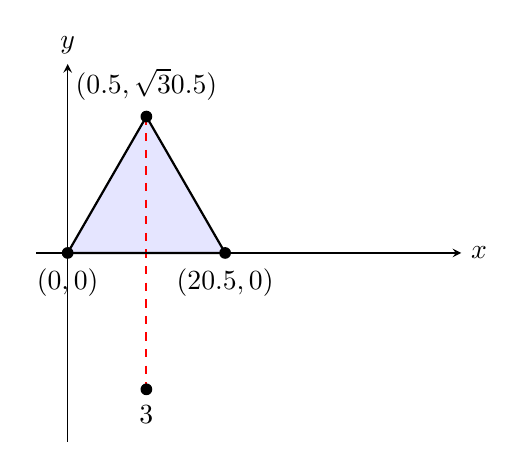
\begin{tikzpicture}[scale=2, >=stealth]
    % Define epsilon (adjust value as needed)
    \def\epsilon{0.5}
    % Calculate coordinates
    \coordinate (0) at (0,0);
    \coordinate (1) at (2*\epsilon, 0);
    \coordinate (2) at (\epsilon, {sqrt(3)*\epsilon});
    \coordinate (3) at (\epsilon, {-sqrt(3)*\epsilon});
    
    % Draw triangle [012]
    \draw[thick, fill=blue!10] (0) -- (1) -- (2) -- cycle;
    
    % Draw point 3 and symmetry line
    \draw[thick, dashed, red] (2) -- (3);
    \node[circle, fill=black, inner sep=1.5pt, label=below:3] at (3) {};
    
    % Label all points
    \foreach \point/\label/\pos in {
        0/{$(0,0)$}/below,
        1/{$(2\epsilon,0)$}/below,
        2/{$(\epsilon,\sqrt{3}\epsilon)$}/above%
    }{
        \node[circle, fill=black, inner sep=1.5pt, label=\pos:\label] at (\point) {};
    }
    
    % Axes (optional, for reference)
    \draw[->, thin] (-0.2,0) -- (2.5,0) node[right] {$x$};
    \draw[->, thin] (0,-1.2) -- (0,1.2) node[above] {$y$};
\end{tikzpicture}
\end{document}